\section{\texttt{simpleStatisticalInverseProblem}}\label{sec:example_sip}

According to the Bayesian paradigm, the unobservable parameters
in a statistical model are treated as random. When no data is available,
a prior distribution is used to quantify our knowledge about the parameter.
When data are available, we can update our prior knowledge using the conditional distribution of parameters, given the data. 
The transition from the prior to the posterior is possible via the Bayes theorem:
\begin{equation*}
\pi_{\text{posterior}}(\boldsymbol{\theta}|\mathbf{d})=\frac{\pi_{\text{prior}}(\boldsymbol{\theta})\pi_{\text{likelihood}}(\mathbf{d}|\boldsymbol{\theta})}{\pi(\mathbf{d})}
\end{equation*}


In this example, suppose a random variable of interest with two parameters $\bv{\theta} \in \mathbb{R}^2$ has a uniform prior distribution, and suppose that a suitable likelihood has normal distribution with mean $\bv{\mu}$ and covariance matrix $\bf{C}$, given by:
\begin{equation}\label{eq-example-mu}
\boldsymbol{\mu} = 
\left(\begin{array}{c}
-1 \\
2
\end{array}\right)
\quad
\text{and}
\quad
\mathbf{C} = 
\left[\begin{array}{cc}
4 & 0 \\
0 & 1
\end{array}\right].
\end{equation}

Therefore, we have: 
\begin{equation*}
\pi_{\text{prior}}(\boldsymbol{\theta}) \varpropto 1
\end{equation*}
and
\begin{equation*}
\pi_{\text{like}}(\boldsymbol{\theta}) \varpropto \exp \left(-\frac{1}{2}\left[(\boldsymbol{\theta}-\boldsymbol{\mu})^T[\mathbf{C}^{-1}](\boldsymbol{\theta}-\boldsymbol{\mu})\right] \right),
\end{equation*}
where
\begin{equation*}
\boldsymbol{\theta} = 
\left(
\begin{array}{c}
\theta_1 \\
\theta_2
\end{array}
\right)\in \mathbb{R}^2.
\end{equation*}
%

Therefore,  posterior PDF is given by:
\begin{equation}\label{eq-example-post}
\pi_{\text{post}}(\boldsymbol{\theta}) \varpropto e^{-\frac{1}{2}\left\{(\boldsymbol{\theta}-\boldsymbol{\mu})^T[\mathbf{C}^{-1}](\boldsymbol{\theta}-\boldsymbol{\mu})\right\}}.
\end{equation}


In this example, we can replace the values for the mean and covariance matrix given in Equation (\ref{eq-example-mu}) into Equation (\ref{eq-example-post}), 
in order to analytically compute both the posterior PDF:
\begin{eqnarray*}\label{eq-example-exact-post}
\pi_{\text{post}}(\boldsymbol{\theta}) & = & \frac{1}{4\pi} \exp\left(-\frac{1}{2}(\boldsymbol{\theta}-\boldsymbol{\mu})^T[\mathbf{C}^{-1}](\boldsymbol{\theta}-\boldsymbol{\mu})\right) \\
                                       & = & \frac{1}{4\pi} \exp\left( -\frac{1}{8}(\theta_1+1)^2 - \frac{1}{2}(\theta_2-2)^2\right), \label{eq-example-exact-joint}
\end{eqnarray*}
and the marginal results for $\theta_1$ and $\theta_2$:
\begin{equation}\label{eq-example-exact-marginal}
\begin{split}
\pi_{\text{post}}(\theta_1) & =  \frac{1}{2\sqrt{2\pi}} \exp\left(-\frac{1}{8}(\theta_1+1)^2 \right), \\
\pi_{\text{post}}(\theta_1) & =  \frac{1}{ \sqrt{2\pi}} \exp\left(-\frac{1}{2}(\theta_2-2)^2 \right). 
\end{split}
\end{equation}



Recall that the posterior PDF given in 
Equation (\ref{eq-example-post}) can be sampled through the expression:
\begin{equation}\label{eq-example-exact-normal}
\boldsymbol{\mu}+\mathbf{C}^{1/2}\mathcal{N}(0,I),
\end{equation}
where $\mathcal{N}(0,I)$ designates a Gaussian joint PDF of zero mean and unit covariance matrix, and
$\mathbf{C}^{1/2}$ is given by:
\begin{equation*}
\mathbf{C}^{1/2} = 
\left[\begin{array}{cc}
2 & 0 \\
0 & 1
\end{array}\right].
\end{equation*}

Thus, in this simple statistical inverse problem, we use QUESO implementation of the Markov chain 
algorithm to sample the posterior \eqref{eq-example-post} via Expression (\ref{eq-example-exact-normal}) and compare the calculated marginal results for $\theta_1$ and $\theta_2$ 
against the analytical formulas given in Equation~(\ref{eq-example-exact-marginal}). 


\paragraph*{Note:} Due to the possibility to compare QUESO sampling algorithms to analytical expressions, this example is also used in the verification procedures and regression tests within QUESO, and it is reproduced in the directory \verb+tests/t02_sip_sfp+.




\subsection{Running the Example}\label{sec:sip-run}
 
To run the executable provided (available after QUESO installation), enter the following commands:
\begin{lstlisting}[label={},caption={}]
$ cd $HOME/LIBRARIES/QUESO-0.47.1/
$ cd examples/simpleStatisticalInverseProblem
$ rm outputData/*
$ ./exSimpleStatisticalInverseProblem_gsl example.inp    
$ matlab
   $ simple_ip_plots      # inside matlab
   $ exit                 # inside matlab
$ ls -l outputData/*.png
 simple_ip_autocorrelation_raw_filt.png  simple_ip_hist_filt.png 
 simple_ip_cdf_filt.png                  simple_ip_hist_raw.png
 simple_ip_cdf_raw.png                   simple_ip_kde_filt.png
 simple_ip_chain_pos_filt.png            simple_ip_kde_raw.png
\end{lstlisting}

As a result, the user should have created several of PNG figures containing marginal posterior PDF, chain positions, histograms, cumulative density distributions and autocorrelation of both parameters. The name of the figure files have been chosen to be informative, as shown in the Listing above. 

It is worth noting presence of an argument passed to the executable in the
example, namely `\verb+example.inp+'. The argument is a input file to be provided to QUESO with options for
the solution of the SIP and/or SFP; and it is always required. Each option in
the input file is related to one (or more) of the QUESO classes, and is
presented throughout Chapter~\ref{ch-classes}. 


\subsection{Example Code}\label{sec:sip-code}

The source code for the example is composed of 5 files:
\texttt{example\_main.C} (Listing \ref{code:sip-main-c}), \linebreak
\texttt{example\_likelihood.h} and \texttt{example\_likelihood.C} (Listings \ref{fig-like-h} and \ref{fig-like-c}),
\texttt{example\_compute.h} and \texttt{example\_compute.C} (Listings \ref{code:sip-compute-h} and \ref{code:sip-compute-c}).


\lstinputlisting[caption=File \texttt{example\_main.C.}, label={code:sip-main-c}, linerange={25-1000}]{../../examples/simpleStatisticalInverseProblem/src/example_main.C}

\lstinputlisting[caption=File \texttt{example\_likelihood.h}., label={fig-like-h}, linerange={25-1000}]{../../examples/simpleStatisticalInverseProblem/src/example_likelihood.h}

\newpage

\lstinputlisting[caption=File \texttt{example\_likelihood.C}., label={fig-like-c}, linerange={25-1000}]{../../examples/simpleStatisticalInverseProblem/src/example_likelihood.C}

\newpage

\lstinputlisting[caption=File \texttt{example\_compute.h.}, label={code:sip-compute-h}, linerange={25-1000}]{../../examples/simpleStatisticalInverseProblem/src/example_compute.h}

\lstinputlisting[caption={File \texttt{example\_compute.C}.}, label={code:sip-compute-c}, linerange={25-1000},numbers=left]{../../examples/simpleStatisticalInverseProblem/src/example_compute.C}
 


\subsection{Input File}\label{sec:sip-input-file}


QUESO reads an input file for solving statistical problems. In the case of a SIP, it expects a list of options for MCMC (or Multilevel),
together with options for QUESO environment; such as the amount of processors to be used and the seed for its random algorithms.
Note that the names of the variables have been designed to be informative:
\begin{description}\vspace{-8pt}
\item[ \texttt{env}:] refers to QUESO environment; \vspace{-8pt}
\item[ \texttt{ip}:] refers to inverse problem;\vspace{-8pt}
\item[ \texttt{mh}:] refers to Metropolis-Hastings;\vspace{-8pt}
\item[ \texttt{dr}:] refers to delayed rejection;\vspace{-8pt}
\item[ \texttt{am}:] refers to adaptive Metropolis;\vspace{-8pt}
\item[ \texttt{rawChain}:] refers to the raw, entire chain; \vspace{-8pt}
\item[ \texttt{filteredChain}:] refers to a filtered chain (related to a specified \texttt{lag});\vspace{-8pt}
\end{description}


The options used for solving this simple SIP are displayed in Listing \ref{code:sip-input-file}.

\lstinputlisting[caption={Options for QUESO library used in application code (Listings \ref{code:sip-main-c}-\ref{code:sip-compute-c}})., 
label={code:sip-input-file},]{../../examples/simpleStatisticalInverseProblem/tests/test_2013_08_26/example.inp}



\subsection{Create your own Makefile}\label{sec:sip-makefile}

Makefiles are special format files that together with the make utility will help one to compile and automatically build and manage projects (programs).  
Listing \ref{code:ip_makefile} presents a Makefile, named `\texttt{Makefile\_sip\_example\_margarida}', that may be used to compile the code and create the executable \verb+simple_sip_example+. Naturally, it must be adapted to the user's settings, i.e., it has to have the correct paths for the user's libraries that have actually been used to compile and install QUESO  (see Sections \ref{sec:Pre_Queso}--\ref{sec:install_Queso_make}).

\lstinputlisting[caption={Makefile for the application code in Listings \ref{code:sip-main-c}-\ref{code:sip-compute-c}},  label={code:ip_makefile},language={bash}]{../../examples/simpleStatisticalInverseProblem/src/Makefile_sip_example_margarida}

Thus, to compile, build and execute the code, the user just needs to run the following commands in the same directory where the files are:
\begin{lstlisting}
$ cd $HOME/LIBRARIES/QUESO-0.47.1/examples/simpleStatisticalInverseProblem/
$ export LD_LIBRARY_PATH=$LD_LIBRARY_PATH:\
  $HOME/LIBRARIES/gsl-1.15/lib/:\
  $HOME/LIBRARIES/boost-1.53.0/lib/:\
  $HOME/LIBRARIES/hdf5-1.8.10/lib:\
  $HOME/LIBRARIES/QUESO-0.47.1/lib 
$ make -f Makefile_example_margarida 
$ ./simple_sip_example example.inp
\end{lstlisting}

The `\verb+export+' instruction above is only necessary if the user has not saved it in his/her \verb+.bashrc+ file. 


\subsection{Data Post-Processing and Visualization}\label{sec:sip-results}


There are a few Matlab-ready commands that are very helpful tools for post-processing the data generated by QUESO when solving statistical inverse problems. This section discusses the results computed by QUESO with the code of Section \ref{sec:sip-code}, and shows how to use Matlab for the post-processing of such results. Only the essential Matlab commands are presented; for the complete/detailed codes, please refer to file '\verb+simple_ip_plots.m+'.

According to the specifications of the input file in Listing~\ref{code:sip-input-file}, a folder named `\verb+outputData+' containing the following files should be created: \verb+display_sub0.txt, ip_filt_chain_sub0.m,+ \verb+ip_raw_chain_sub0.m, sipOutput_sub0.m, ip_filt_chain.m, ip_raw_chain.m+
% \begin{verbatim}
% display_sub0.txt
% ip_filt_chain_sub0.m
% ip_raw_chain_sub0.m
% sipOutput_sub0.m
% ip_filt_chain.m
% ip_raw_chain.m
% \end{verbatim}


The code bellow shows how to load the data provided by QUESO during the solution process of the SIP described, in the form of 
chains of positions.

\begin{lstlisting}[caption={Matlab code for loading the data in both raw and filtered chains of the SIP, by calling the file \texttt{simple\_ip\_plots.m}.}]
% inside Matlab
>> clear all
>> simple_ip_plots
\end{lstlisting}


\subsubsection{Autocorrelation Plots}

The code presented in Listing \ref{matlab:simple_sip_autocorr} uses Matlab function \verb+autocorr+ to generate Figure \ref{fig:simple_sip_autocorrelation_raw_filt}
which presents the autocorrelation of the parameters $\theta_1$ and $\theta_2$ in both cases: raw and filtered chain. 

\begin{lstlisting}[label=matlab:simple_sip_autocorr,caption={Matlab code for the autocorrelation plots depicted in Figure \ref{fig:simple_sip_autocorrelation_raw_filt}.}]
% inside Matlab
% theta_1
>> nlags=10;
>> [ACF_raw, lags] = autocorr(ip_mh_rawChain_unified(:,1), nlags, 0);
>> [ACF_filt, lags] = autocorr(ip_mh_filtChain_unified(:,1), nlags, 0);
>> [ACF_raw2, lags2] = autocorr(ip_mh_rawChain_unified(:,2), nlags, 0);
>> [ACF_filt2, lags3] = autocorr(ip_mh_filtChain_unified(:,2), nlags, 0);
>> plot(lags,ACF_raw,'b--*',lags,ACF_filt,'b*-',lags2,ACF_raw2,'g--*',lags2,ACF_filt2,'g*-','linewidth',3);
>> h=legend('\theta_1, raw chain','\theta_1, filtered chain','\theta_2, raw chain','\theta_2, filtered chain','location','northeast');
\end{lstlisting}

\begin{figure}[htpb]
\centering
%\subfloat[$\theta_1$]{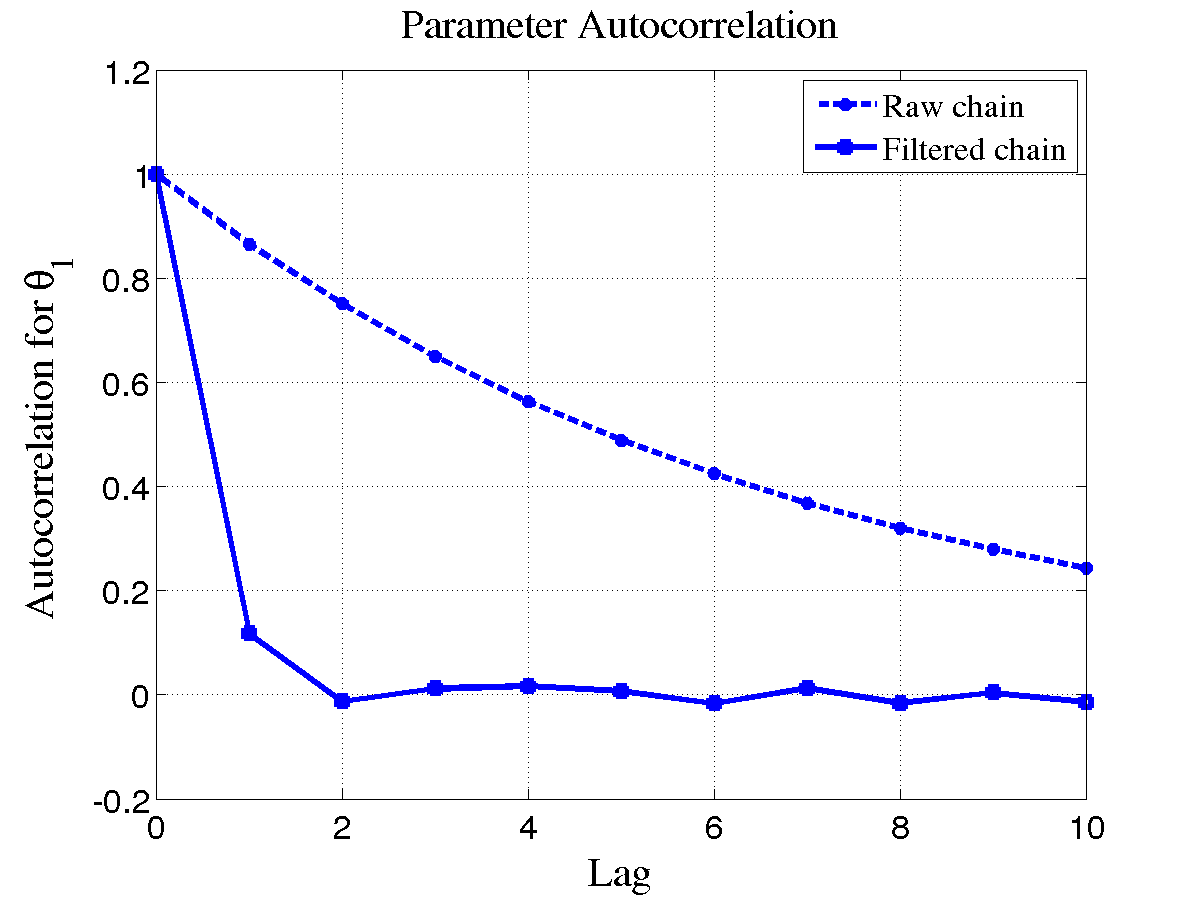
\includegraphics[scale=0.35]{figs/simple_ip_autocorrelation_raw_filt_theta1.png}}
%\subfloat[$\theta_2$]{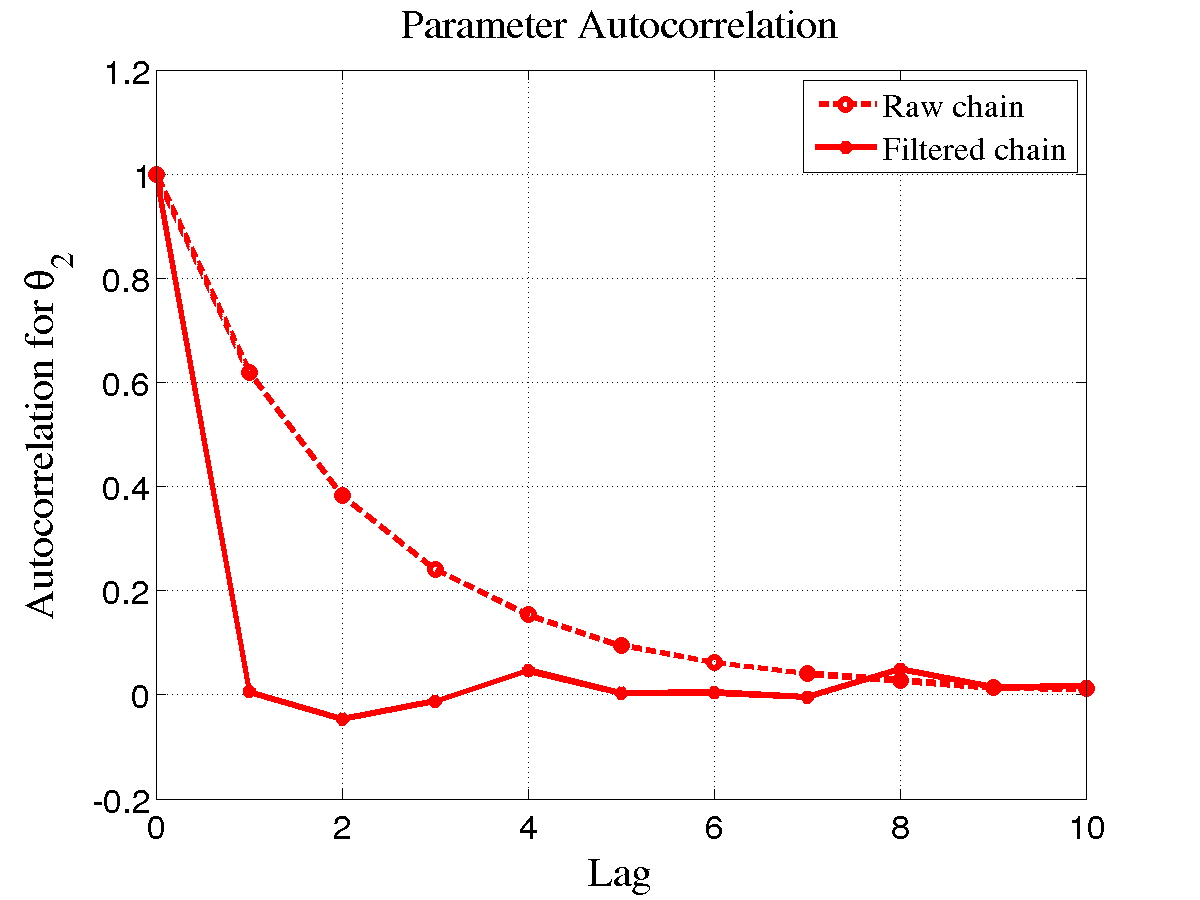
\includegraphics[scale=0.35]{figs/simple_ip_autocorrelation_raw_filt_theta2.png}}
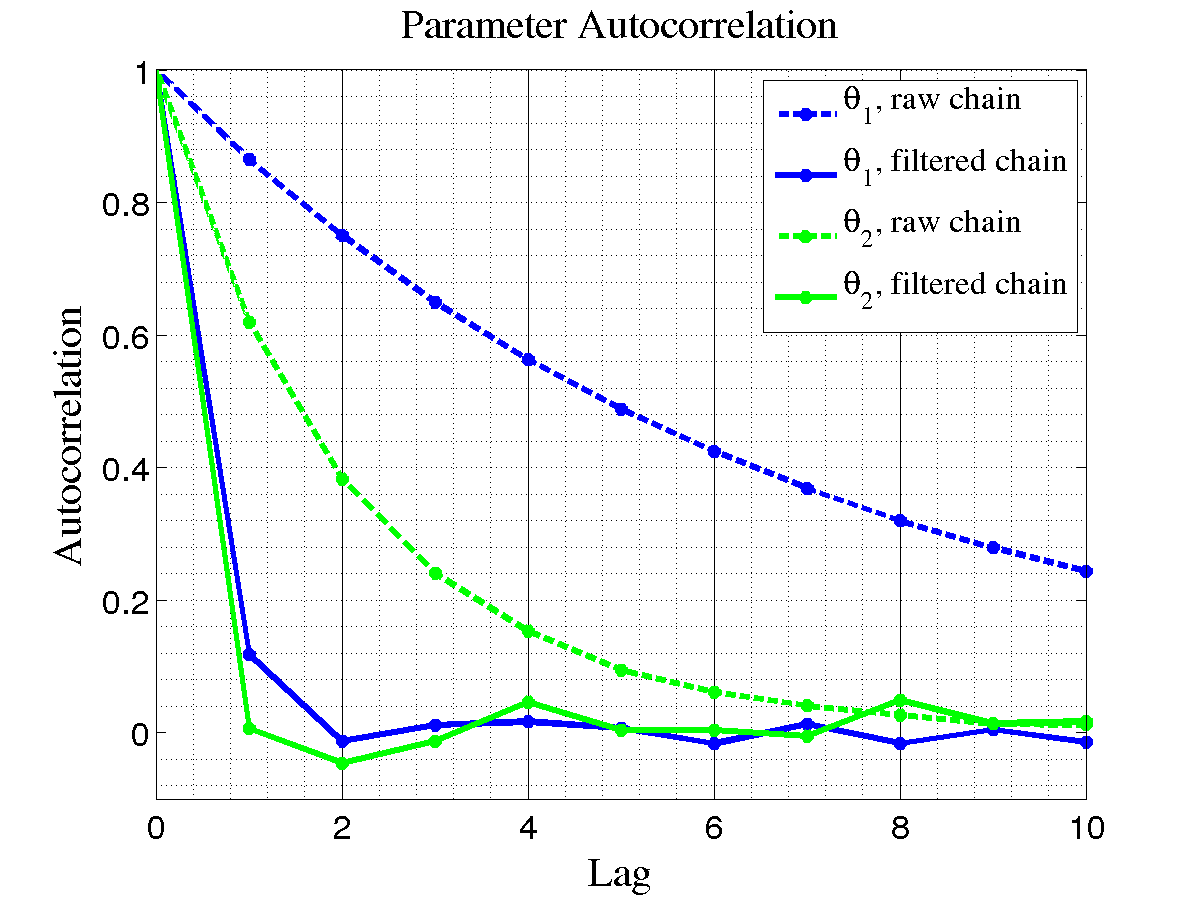
\includegraphics[scale=0.35]{figs/simple_ip_autocorrelation_raw_filt.png}
\vspace{-10pt}
\caption{
Autocorrelation plots obtained with QUESO for the SIP. }
\label{fig:simple_sip_autocorrelation_raw_filt}
\end{figure}


\subsubsection{KDE Plots}

Matlab function \verb+[f,xi] = ksdensity(x)+ (kernel smoothing density estimate) computes a probability density estimate of the sample in the vector \texttt{x}. \texttt{f} is the vector of density values evaluated at the points in \texttt{xi}. The estimate is based on a normal kernel function, using a window parameter (`width') that is a function of the number of points in \texttt{x}. The density is evaluated at 100 equally spaced points that cover the range of the data in x.  In order to estimate the KDE of the parameters, it is used together with the option `\verb+pdf+'. 

\begin{lstlisting}[label=matlab:ip_kde,caption={Matlab code for the KDE plots displayed in the left of Figure \ref{fig:simple_sip_kde}.}]
% Inside Matlab
% Raw chain
>> [f,x] = ksdensity(ip_mh_rawChain_unified(:,1),'function','pdf');
>> [f2,x2] = ksdensity(ip_mh_rawChain_unified(:,2),'function','pdf');
>> x_p1=sort(ip_mh_rawChain_unified(:,1)); %analytical
>> f_p1=(exp(-(x_p1+1).*(x_p1+1)/8))/2/sqrt(2*pi);
>> x_p2=sort(ip_mh_rawChain_unified(:,1));
>> f_p2=(exp(-(x_p2-2).*(x_p2-2)/2))/sqrt(2*pi);
>> plot(x,f,'b',x2,f2,'g','linewidth',4);
>> hold;
>> plot(x_p1,f_p1,'--k',x_p2,f_p2,'-k','linewidth',2);
>> h=legend('\theta_1', '\theta_2', 'analytical (\theta_1)', 'analytical (\theta_2)', 'location', 'northwest');
\end{lstlisting}

% \begin{lstlisting}[label=matlab:ip_kde,caption={Matlab code for the KDE plots displayed in Figure \ref{fig:simple_sip_kde}.}]
% % inside Matlab
% % theta_1
% >> [f,xi] = ksdensity(ip_mh_rawChain_unified(:,1),'function','pdf');
% >> x=ip_mh_rawChain_unified(:,1);
% >> x=sort(x);
% >> plot(x,(exp(-(x+1).*(x+1)/8))/2/sqrt(2*pi),'--k',xi,f,'-b','linewidth',3);
% >> title('Parameter Kernel Density Estimation (raw chain)','fontname', 'Times', 'fontsize',20);
% >> ylabel('Posterior marginal PDF','fontname', 'Times', 'fontsize',20);
% >> xlabel('\theta_1','fontname', 'Times', 'fontsize',20);
% >> h=legend('Analytical','QUESO','location','northeast');
% 
% % theta_2
% >> fprintf(1,' Plotting KDE - raw  <press any key>\n');
% >> [f,xi] = ksdensity(ip_mh_rawChain_unified(:,2),'function','pdf');
% >> x=ip_mh_rawChain_unified(:,2);
% >> x=sort(x);
% >> plot(x,(exp(-(x-2).*(x-2)/2))/sqrt(2*pi),'--k',xi,f,'-r','linewidth',3);
% >> title('Parameter Kernel Density Estimation (raw chain)','fontname', 'Times', 'fontsize',20);
% >> ylabel('Posterior marginal PDF','fontname', 'Times', 'fontsize',20);
% >> xlabel('\theta_2','fontname', 'Times', 'fontsize',20);
% >> h=legend('Analytical','QUESO','location','northeast');
% \end{lstlisting}

%Figure \ref{fig:sip_gravity_kde_raw} is created by using Matlab commands presented in Listing \ref{matlab:kde} above.
\begin{figure}[htpb]
\centering 
% \subfloat[]{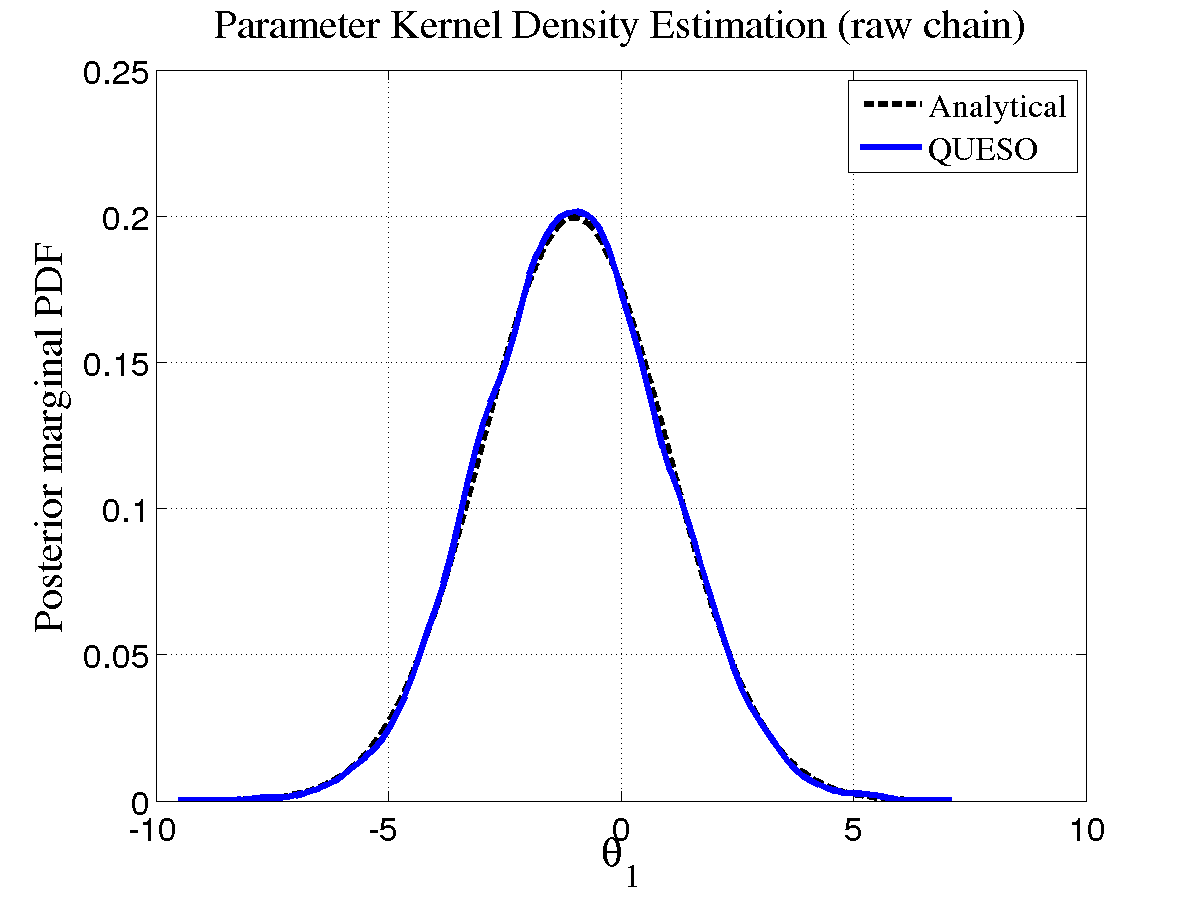
\includegraphics[scale=0.35]{figs/simple_ip_kde_theta1.png}}
% \subfloat[]{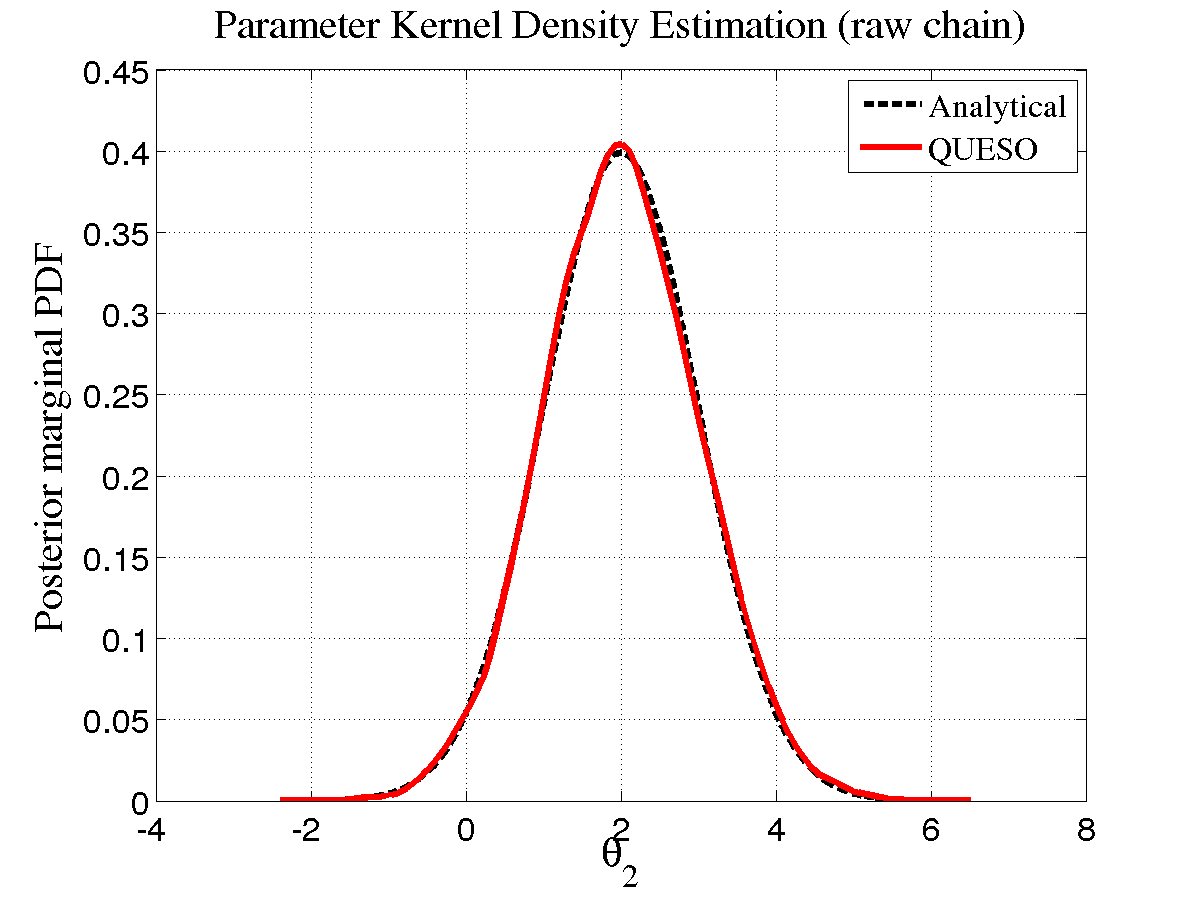
\includegraphics[scale=0.35]{figs/simple_ip_kde_theta2.png}}
\subfloat[Raw chain]{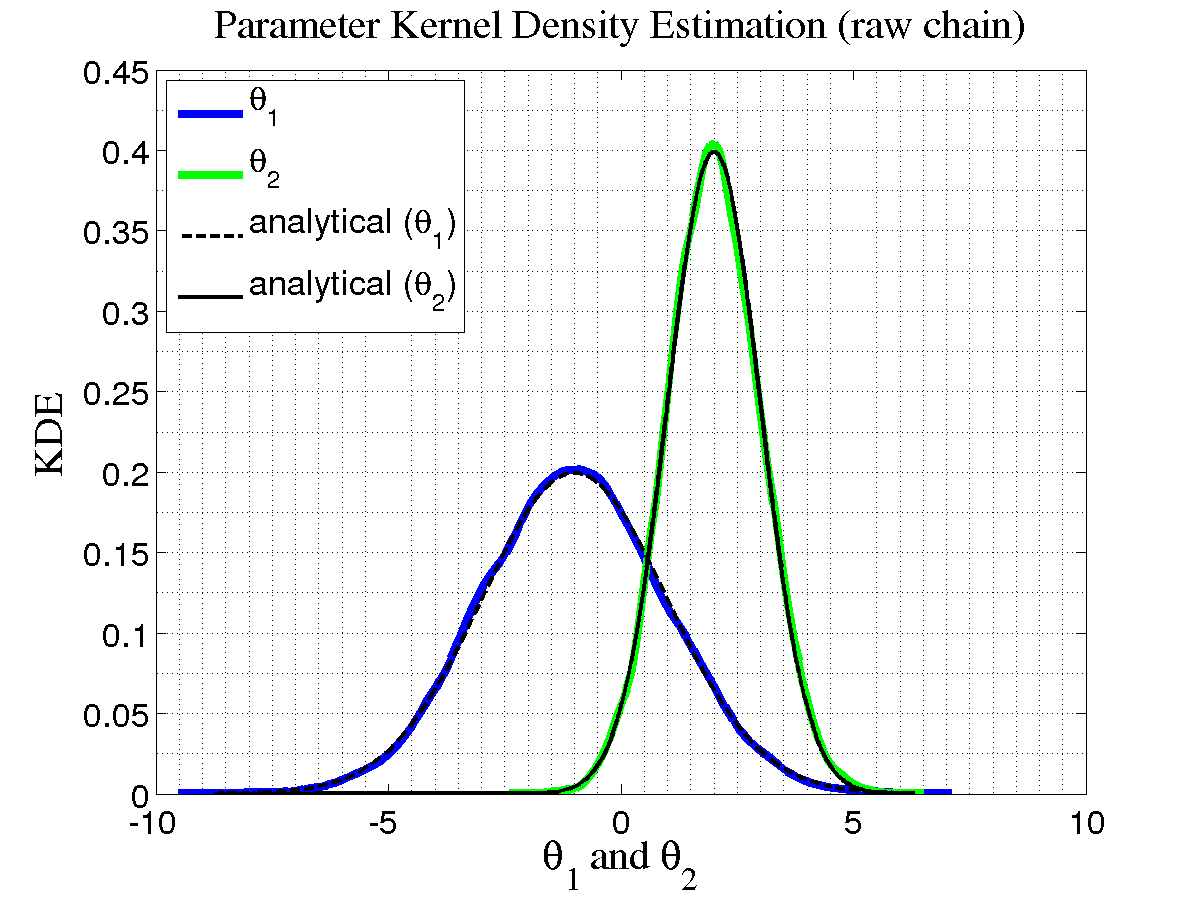
\includegraphics[scale=0.35]{figs/simple_ip_kde_raw.png}}
\subfloat[Filtered chain]{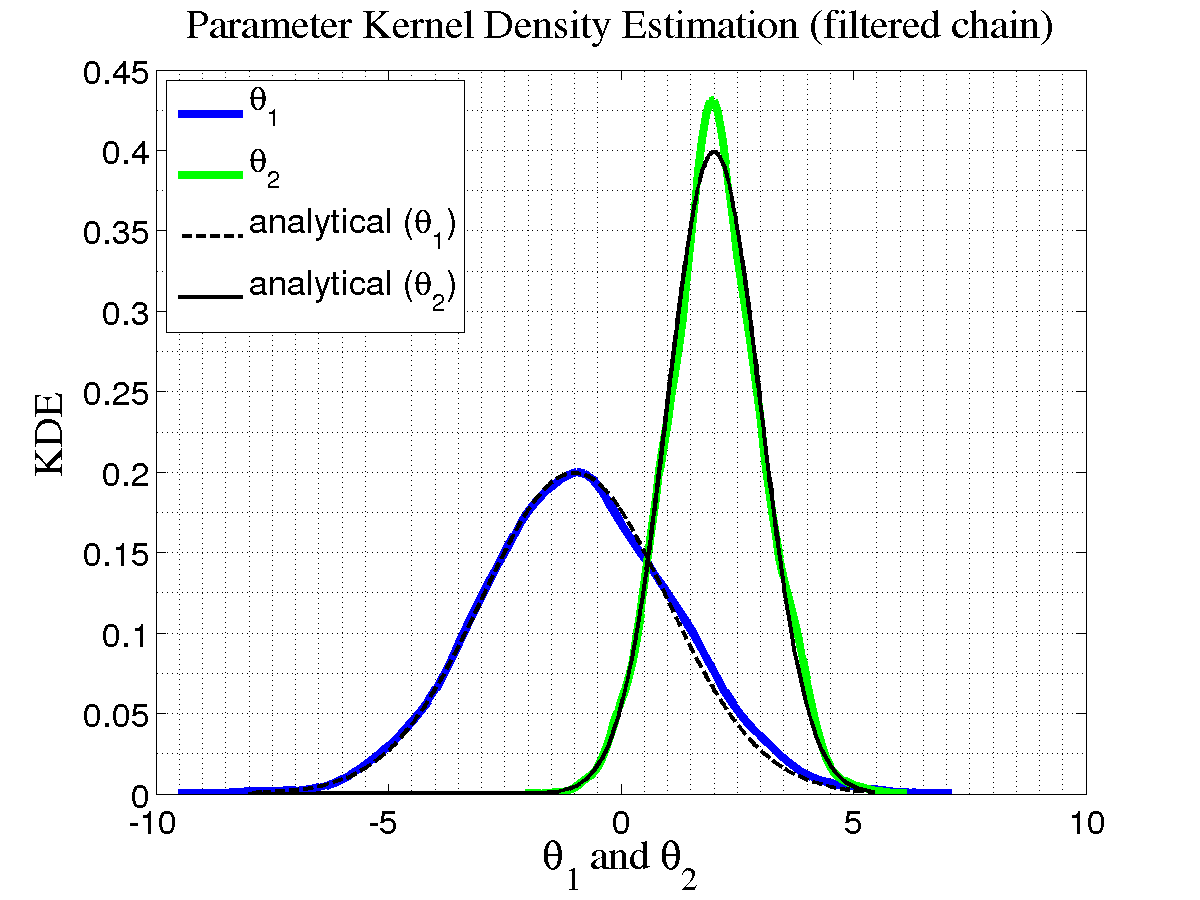
\includegraphics[scale=0.35]{figs/simple_ip_kde_filt.png}}
\vspace*{-10pt}
\caption{Kernel Density Estimation. QUESO results for estimation of the KDE of $\theta_1$ and $\theta_2$ are plotted against the analytical expressions $\pi_{\text{post}}(\theta_1)  =  \frac{1}{2\sqrt{2\pi}} \exp\left(-\frac{1}{8}(\theta_1+1)^2 \right)$  and $\pi_{\text{post}}(\theta_2)  =  \frac{1}{ \sqrt{2\pi}} \exp\left(-\frac{1}{2}(\theta_2-2)^2 \right)$, respectively.}
\label{fig:simple_sip_kde}
\end{figure}


\subsubsection{Covariance and Correlation Matrices}

Matlab function \verb+cov+ calculates the covariance matrix for a data matrix (where each column represents a separate quantity), 
and \verb+corr+ calculates the correlation matrix.

Listing \ref{matlab:cov_matrix} presents the Matlab steps for calculating the covariance and correlation matrices for the parameters $\theta_1$ and $\theta_2$.

\newpage

\begin{lstlisting}[label=matlab:ip_cov_matrix,caption={Matlab code for finding covariance and correlation matrices.}]
% inside Matlab
>> cov_matrix_theta1_theta2 = cov(ip_mh_rawChain_unified)

cov_matrix_theta1_theta2 =

    3.8729    0.0259
    0.0259    1.0050
    
>> corr_matrix_theta1_theta2 = corr(ip_mh_rawChain_unified)

corr_matrix_theta1_theta2 =

    1.0000    0.0132
    0.0132    1.0000    
\end{lstlisting}

